\documentclass[border=6pt]{standalone}
\usepackage{tikz}
\usepackage{amsmath}
\usetikzlibrary{positioning,arrows.meta,calc,fit,backgrounds,shapes.geometric,decorations.pathreplacing}
\definecolor{inkc}{HTML}{171A22}
\definecolor{mutedc}{HTML}{5B6274}
\definecolor{hairc}{HTML}{C9CEDA}
\definecolor{surfc}{HTML}{F2F4F8}
\definecolor{scalec}{HTML}{2E45A8}   % blue  = scale path
\definecolor{elemc}{HTML}{A65A18}    % ochre = element path
\definecolor{costc}{HTML}{B3261E}    % red   = the expensive operator
\definecolor{freec}{HTML}{1E6F4C}    % green = free / shift-only
% text macro for the small monospace annotations inside nodes
\newcommand{\dt}[1]{{\tiny\ttfamily\textcolor{mutedc}{#1}}}
\tikzset{
  blk/.style   ={draw=inkc,line width=.6pt,rounded corners=1.5pt,fill=white,
                 inner sep=4pt,align=center,font=\scriptsize},
  op/.style    ={blk,fill=surfc},
  mul/.style   ={blk,draw=costc,line width=1pt,fill=costc!7,text=costc},
  free/.style  ={blk,draw=freec,fill=freec!7,text=freec},
  scaleb/.style={blk,draw=scalec,fill=scalec!7,text=scalec},
  elemb/.style ={blk,draw=elemc,fill=elemc!7,text=elemc},
  dat/.style   ={font=\scriptsize\ttfamily,text=mutedc},
  lbl/.style   ={font=\scriptsize,text=mutedc,align=center},
  ttl/.style   ={font=\small\bfseries,text=inkc},
  ar/.style    ={-{Stealth[length=4pt,width=3pt]},draw=inkc,line width=.5pt},
  arS/.style   ={ar,draw=scalec},
  arE/.style   ={ar,draw=elemc},
}

\begin{document}
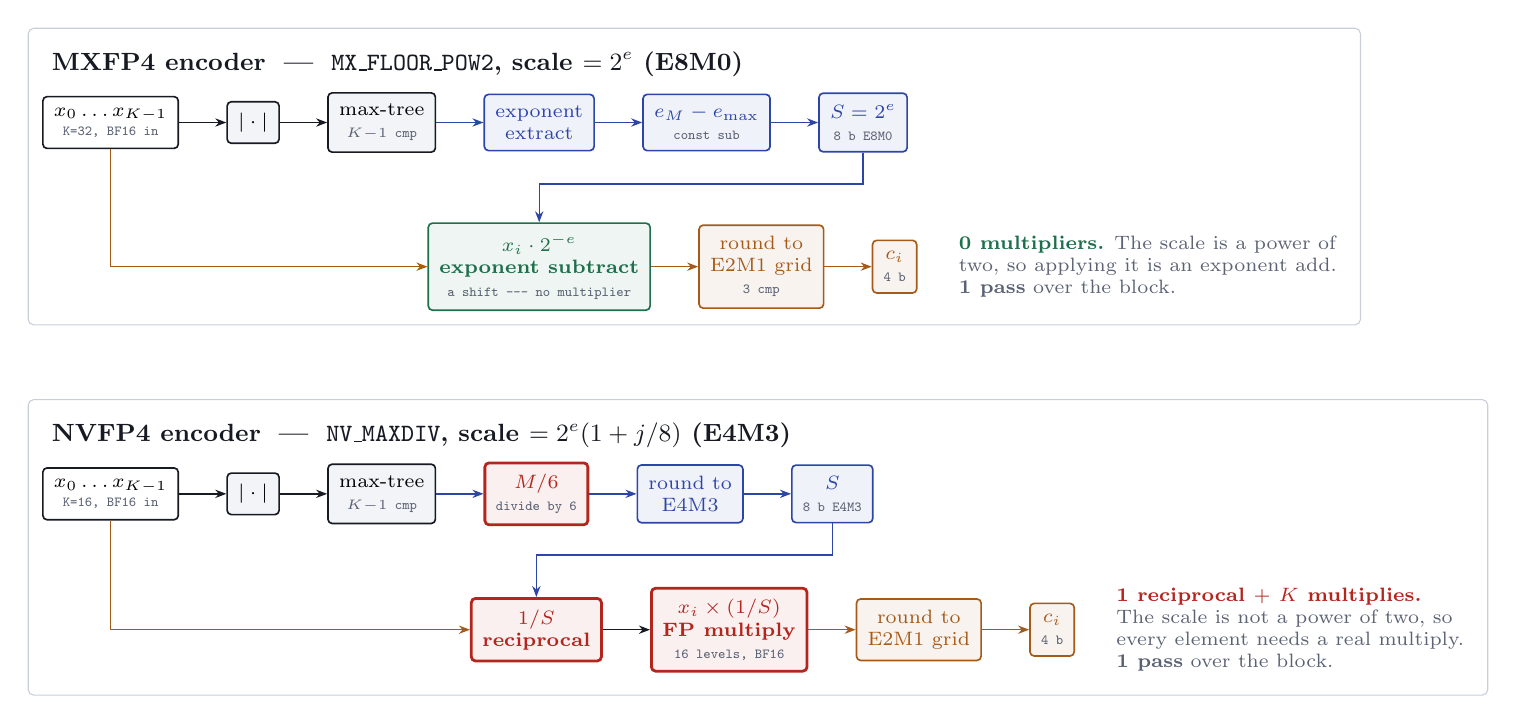
\begin{tikzpicture}[node distance=6mm]

% ============================ MXFP4 =====================================
\node[ttl] (t1) {MXFP4 encoder \;---\; \texttt{MX\_FLOOR\_POW2}, scale $=2^{e}$ (E8M0)};
\node[blk,below=4mm of t1.west,anchor=north west] (x1) {$x_0\dots x_{K-1}$\\[-1pt]\dt{K=32, BF16 in}};
\node[op,right=of x1]   (abs1) {$|\cdot|$};
\node[op,right=of abs1] (max1) {max-tree\\\dt{$K{-}1$ cmp}};
\node[scaleb,right=of max1] (ee1) {exponent\\extract};
\node[scaleb,right=of ee1]  (sub1) {$e_M-e_{\max}$\\\dt{const sub}};
\node[scaleb,right=of sub1] (s1) {$S=2^{e}$\\\dt{8 b E8M0}};
\draw[ar](x1)--(abs1); \draw[ar](abs1)--(max1); \draw[arS](max1)--(ee1);
\draw[arS](ee1)--(sub1); \draw[arS](sub1)--(s1);

\node[free,below=9mm of ee1] (sh1) {$x_i \cdot 2^{-e}$\\\textbf{exponent subtract}\\\dt{a shift --- no multiplier}};
\node[elemb,right=of sh1] (rd1) {round to\\E2M1 grid\\\dt{3 cmp}};
\node[elemb,right=of rd1] (c1) {$c_i$\\\dt{4 b}};
\draw[arE]($(x1.south)+(0,0)$)|-(sh1.west);
\draw[arS](s1.south)--++(0,-4mm)-|(sh1.north);
\draw[arE](sh1)--(rd1); \draw[arE](rd1)--(c1);
\node[lbl,right=4mm of c1,align=left] (n1)
  {\textcolor{freec}{\textbf{0 multipliers.}} The scale is a power of\\
   two, so applying it is an exponent add.\\
   \textbf{1 pass} over the block.};

% ============================ NVFP4 =====================================
\node[ttl,anchor=north west] (t2) at ($(x1.north west|-sh1.south)+(0,-13mm)$)
  {NVFP4 encoder \;---\; \texttt{NV\_MAXDIV}, scale $=2^{e}(1+j/8)$ (E4M3)};
\node[blk,below=4mm of t2.west,anchor=north west] (x2) {$x_0\dots x_{K-1}$\\[-1pt]\dt{K=16, BF16 in}};
\node[op,right=of x2]   (abs2) {$|\cdot|$};
\node[op,right=of abs2] (max2) {max-tree\\\dt{$K{-}1$ cmp}};
\node[mul,right=of max2] (div2) {$M/6$\\\dt{divide by 6}};
\node[scaleb,right=of div2] (rq2) {round to\\E4M3};
\node[scaleb,right=of rq2] (s2) {$S$\\\dt{8 b E4M3}};
\draw[ar](x2)--(abs2); \draw[ar](abs2)--(max2); \draw[arS](max2)--(div2);
\draw[arS](div2)--(rq2); \draw[arS](rq2)--(s2);

\node[mul,below=9mm of div2] (rec2) {$1/S$\\\textbf{reciprocal}};
\node[mul,right=of rec2] (mul2) {$x_i \times (1/S)$\\\textbf{FP multiply}\\\dt{16 levels, BF16}};
\node[elemb,right=of mul2] (rd2) {round to\\E2M1 grid};
\node[elemb,right=of rd2] (c2) {$c_i$\\\dt{4 b}};
\draw[arS](s2.south)--++(0,-4mm)-|(rec2.north);
\draw[arE]($(x2.south)$)|-(rec2.west);
\draw[ar](rec2)--(mul2); \draw[arE](mul2)--(rd2); \draw[arE](rd2)--(c2);
\node[lbl,right=4mm of c2,align=left] (n2)
  {\textcolor{costc}{\textbf{1 reciprocal $+$ $K$ multiplies.}}\\
   The scale is not a power of two, so\\
   every element needs a real multiply.\\
   \textbf{1 pass} over the block.};

\begin{scope}[on background layer]
  \node[fit=(t1)(n1)(c1)(sh1),draw=hairc,rounded corners=2pt,inner sep=5pt]{};
  \node[fit=(t2)(n2)(c2)(rec2),draw=hairc,rounded corners=2pt,inner sep=5pt]{};
\end{scope}
\end{tikzpicture}
\end{document}
